\documentclass[12pt]{article}

\usepackage[margin=1in]{geometry}
\usepackage{graphicx}
\usepackage{setspace}
\usepackage[htt]{hyphenat}
\graphicspath{{./}}

\begin{document}
	\onehalfspace
	\begin{center}
		\begin{large} Computer Networks PA \#1 \end{large}
	\end{center}
	
	\hfill Charlie Coleman
		
	\hfill Spent 8 hours. Started on February 23rd.\\
	
	To run these tests, I altered the parameters (message size and delay) within the \texttt{part2-client.py} file, leaving the server running for the duration of the experiment. RTT was calculated by the code for each message and helg in an array, then the mean was calculated after all probes were sent. Throughput was calculated by measuring the time spent sending/recieving all probes, calculating the total data transferred, then calculating the throughput of the connection. For timing, \texttt{time.time()} was used for all measurements. This provided microsecond accuracy. All final calculations were recorded to the nanosecond.
	
	Using my client/server code to test the RTT of a TCP packet, I found that the RTT increased as the packet size increased. I hypothesize that this is because there is a higher chance of data loss with more bytes, and because there is some effect of the console printing out the echo'd data. When some server delay is added, it makes up the vast majority of the RTT, as the RTT is on the order of tens of microseconds. The trend in the RTT with server delay is less pronounced, but this may be due to the fact that the RTT variations are close to the maximum accuracy of the measurements.
	
	When testing the throughput of the connection, I found that it decreased as the message size increased. This was counter to my initial presumptions, as I assumed that sending more data at a time would improve throughput. I hypothesize that this is due to initial error chance, similar to the RTT testing, and due to the printing of the echo'd data. The trend flips when a delay is added to the server, and the throughput begins to scale very linearly with the message size. This is due to the fact that the RTT is now nearly negligible compared to the server delay, so the throughput is now a function of the message size.
	
	I ran all of the tests for these graphs on my home computer, connected to the SLU wired network. This PC is running  Linux. I ran the RTT tests with 2000 probes each, and the throughput tests with 200 probes each. Each test was run with the 6 different message sizes at 3 different delays (0ms, 10ms, and 100ms). 
	
	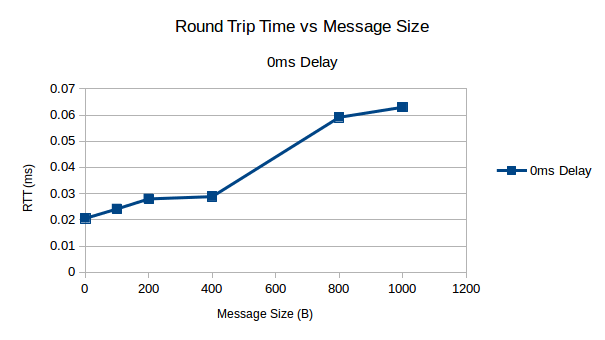
\includegraphics[width=.5\textwidth]{rtt0ms}
	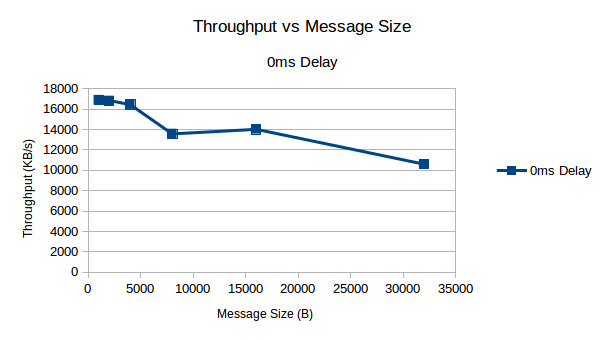
\includegraphics[width=.5\textwidth]{tput0ms}
	
	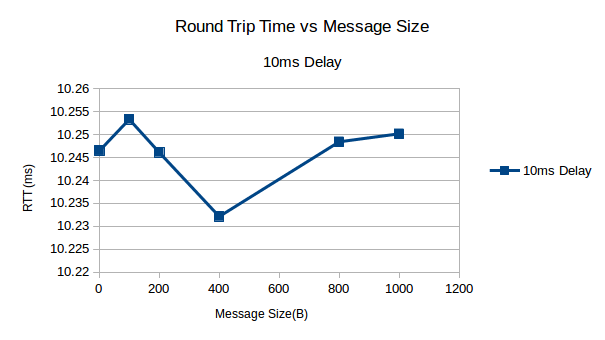
\includegraphics[width=.5\textwidth]{rtt10ms}
	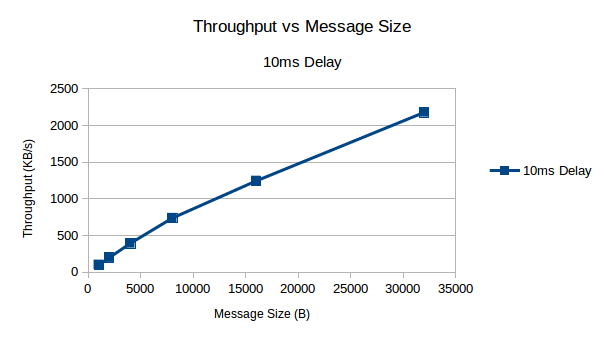
\includegraphics[width=.5\textwidth]{tput10ms}
	
	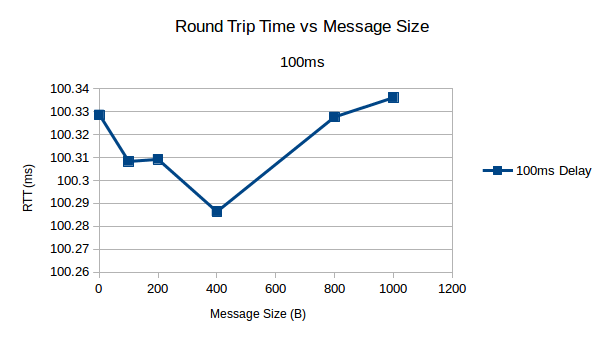
\includegraphics[width=.5\textwidth]{rtt100ms}
	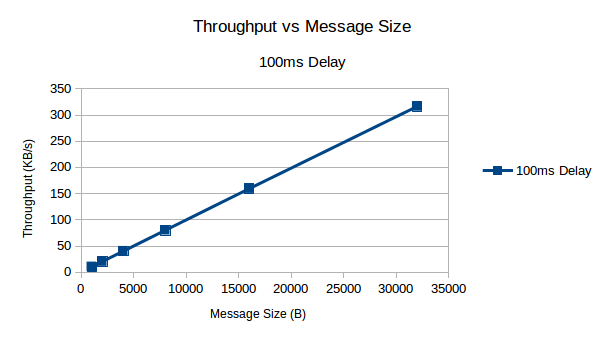
\includegraphics[width=.5\textwidth]{tput100ms}
\end{document}